\documentclass{standalone}

\usepackage{../../core}

\def\ystep{0.1795in}
\def\yoff{0.01in}
\def\yg{17.9}
\def\xgstep{0.35}

\begin{document}
\begin{tikzpicture}[
  C/.style={circle,
            draw=darkcolor,
            line width=0.7pt,
            text=textcolor,
            inner sep=2pt
            },
  G/.style={anchor=south,
            text=textcolor,
            inner sep=0pt
            },
  M/.style={anchor=south west,
            draw=darkcolor,
            thin,
            inner sep=1pt
            },
  N/.style={text=textcolor,
            anchor=south east,
            inner sep=0pt,
            xshift=-2.43in
            }
]

\node[C] at (0.68,19.5) {\large \strut $\*u$};
\node[C] at (4.58,19.5) {\large \strut $\*w$};
\node[C] at (10.4,19.5) {\large \strut $\*v$};

\node[G,align=center] at (2.12, \yg) {\sffamily \strut R\textsubscript{1}\\\sffamily \strut R\textsubscript{4}};
\node[G] at (2.12+1*\xgstep, \yg) {\sffamily \strut R\textsubscript{2}};
\node[G] at (2.12+2*\xgstep, \yg) {\sffamily \strut R\textsubscript{3}};
\node[G] at (2.12+3*\xgstep, \yg) {\sffamily \strut R\textsubscript{5}};
\node[G] at (2.12+4*\xgstep, \yg) {\sffamily \strut R\textsubscript{6}};
\node[G,align=center] at (2.12+5*\xgstep, \yg) {\sffamily \strut R\textsubscript{7}\\\sffamily \strut R\textsubscript{9}};
\node[G] at (2.12+6*\xgstep, \yg) {\sffamily \strut R\textsubscript{8}};
\node[G] at (2.12+7*\xgstep, \yg) {\sffamily \strut R\textsubscript{10}};
\node[G] at (2.12+8*\xgstep, \yg) {\sffamily \strut R\textsubscript{11}};

\node[G] at (7.97, \yg) {\sffamily \strut A\textsubscript{1}};
\node[G] at (7.97+1*\xgstep, \yg) {\sffamily \strut A\textsubscript{2}};
\node[G] at (7.97+2*\xgstep, \yg) {\sffamily \strut A\textsubscript{3}};
\node[G,align=center] at (7.97+3*\xgstep, \yg) {\sffamily \strut A\textsubscript{4}\\\sffamily \strut A\textsubscript{7}};
\node[G] at (7.97+4*\xgstep, \yg) {\sffamily \strut A\textsubscript{5}};
\node[G] at (7.97+5*\xgstep, \yg) {\sffamily \strut A\textsubscript{6}};
\node[G] at (7.97+6*\xgstep, \yg) {\sffamily \strut A\textsubscript{8}};
\node[G] at (7.97+7*\xgstep, \yg) {\sffamily \strut A\textsubscript{9}};
\node[G] at (7.97+8*\xgstep, \yg) {\sffamily \strut A\textsubscript{10}};
\node[G] at (7.97+9*\xgstep, \yg) {\sffamily \strut A\textsubscript{11}};
\node[G,align=center] at (7.97+10*\xgstep, \yg) {\sffamily \strut A\textsubscript{12}\\\sffamily \strut A\textsubscript{13}\\\sffamily \strut A\textsubscript{14}};

\node[M] at (0,0) {
\includegraphics[height=7in]{mat_brca_u.png}};
\node[M] at (1.9,0) {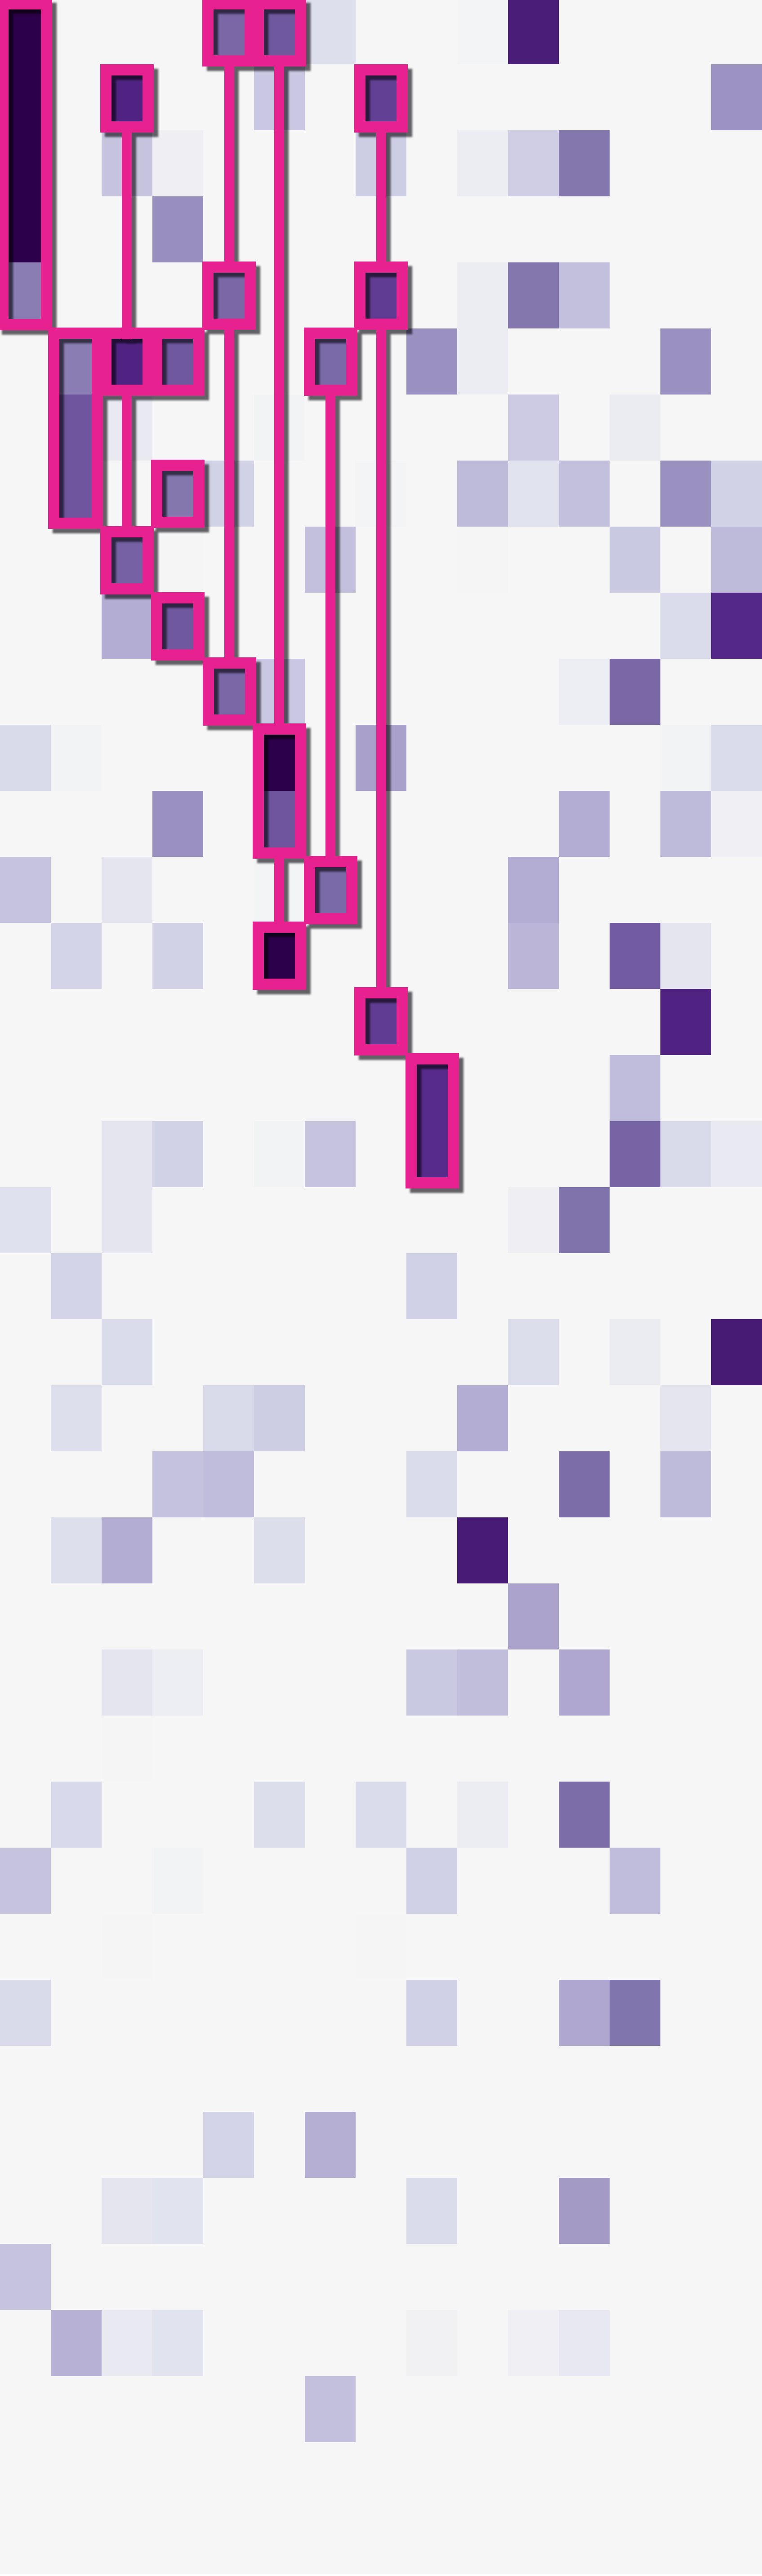
\includegraphics[height=7in]{mat_brca_w_annotated.png}};
\node[M] at (7.75,0) {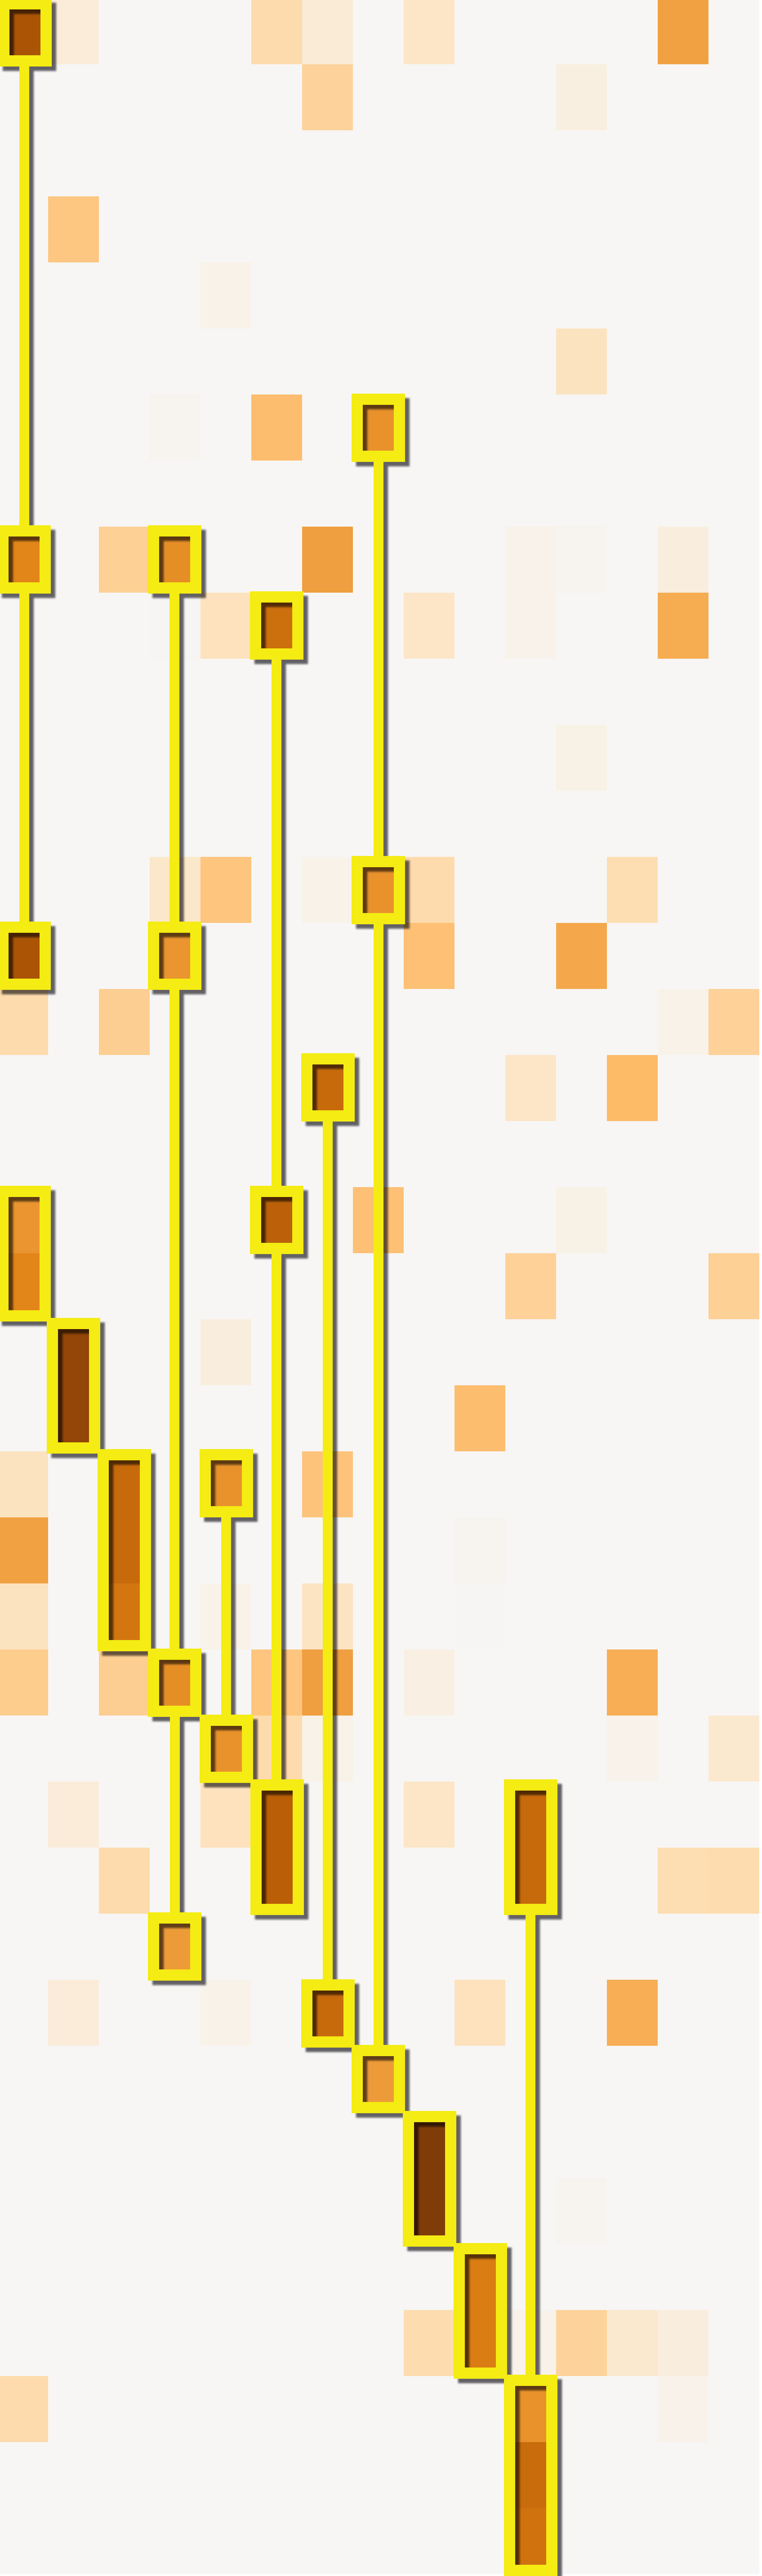
\includegraphics[height=7in]{mat_brca_v_annotated.png}};

\node[N,yshift=38*\ystep-\yoff] at (current page.south) {\sffamily \strut TP53};
\node[N,yshift=37*\ystep-\yoff] at (current page.south) {\sffamily \strut GATA3};
\node[N,yshift=36*\ystep-\yoff] at (current page.south) {\sffamily \strut CTCF};
\node[N,yshift=35*\ystep-\yoff] at (current page.south) {\sffamily \strut CADPS};
\node[N,yshift=34*\ystep-\yoff] at (current page.south) {\sffamily \strut CDH1};
\node[N,yshift=33*\ystep-\yoff] at (current page.south) {\sffamily \strut PIK3CA};
\node[N,yshift=32*\ystep-\yoff] at (current page.south) {\sffamily \strut MCL1(A)};
\node[N,yshift=31*\ystep-\yoff] at (current page.south) {\sffamily \strut AKT1};
\node[N,yshift=30*\ystep-\yoff] at (current page.south) {\sffamily \strut ING5(D)};
\node[N,yshift=29*\ystep-\yoff] at (current page.south) {\sffamily \strut PTEN(D)};
\node[N,yshift=28*\ystep-\yoff] at (current page.south) {\sffamily \strut MAP2K4};
\node[N,yshift=27*\ystep-\yoff] at (current page.south) {\sffamily \strut MAP3K1};
\node[N,yshift=26*\ystep-\yoff] at (current page.south) {\sffamily \strut ENSG\ldots247765};
\node[N,yshift=25*\ystep-\yoff] at (current page.south) {\sffamily \strut ING1,ERCC5(A)};
\node[N,yshift=24*\ystep-\yoff] at (current page.south) {\sffamily \strut MYC(A)};
\node[N,yshift=23*\ystep-\yoff] at (current page.south) {\sffamily \strut STK11,TCF3(D)};
\node[N,yshift=22*\ystep-\yoff] at (current page.south) {\sffamily \strut PAX7,SDHB(D)};
\node[N,yshift=21*\ystep-\yoff] at (current page.south) {\sffamily \strut RUNX1};
\node[N,yshift=20*\ystep-\yoff] at (current page.south) {\sffamily \strut FAM208B(A)};
\node[N,yshift=19*\ystep-\yoff] at (current page.south) {\sffamily \strut ARHGAP35(D)};
\node[N,yshift=18*\ystep-\yoff] at (current page.south) {\sffamily \strut CCND1(A)};
\node[N,yshift=17*\ystep-\yoff] at (current page.south) {\sffamily \strut INTS4(A)};
\node[N,yshift=16*\ystep-\yoff] at (current page.south) {\sffamily \strut TUBD1(A)};
\node[N,yshift=15*\ystep-\yoff] at (current page.south) {\sffamily \strut ERBB2(A)};
\node[N,yshift=14*\ystep-\yoff] at (current page.south) {\sffamily \strut BRCA1(D)};
\node[N,yshift=13*\ystep-\yoff] at (current page.south) {\sffamily \strut KDM5A(A)};
\node[N,yshift=12*\ystep-\yoff] at (current page.south) {\sffamily \strut FOXA1(A)};
\node[N,yshift=11*\ystep-\yoff] at (current page.south) {\sffamily \strut DUX4(D)};
\node[N,yshift=10*\ystep-\yoff] at (current page.south) {\sffamily \strut DUX4,FAT1,\ldots};
\node[N,yshift=9*\ystep-\yoff] at (current page.south) {\sffamily \strut PLCL2};
\node[N,yshift=8*\ystep-\yoff] at (current page.south) {\sffamily \strut TRIM33,NRAS,\ldots};
\node[N,yshift=7*\ystep-\yoff] at (current page.south) {\sffamily \strut NLRC5};
\node[N,yshift=6*\ystep-\yoff] at (current page.south) {\sffamily \strut ZNF703(A)};
\node[N,yshift=5*\ystep-\yoff] at (current page.south) {\sffamily \strut IKBKB(A)};
\node[N,yshift=4*\ystep-\yoff] at (current page.south) {\sffamily \strut DDX10,POU2AF1,\ldots};
\node[N,yshift=3*\ystep-\yoff] at (current page.south) {\sffamily \strut SIRT3,CARS,\ldots};
\node[N,yshift=2*\ystep-\yoff] at (current page.south) {\sffamily \strut LOC283050(A)};
\node[N,yshift=1*\ystep-\yoff] at (current page.south) {\sffamily \strut DNAH7};
\node[N,yshift=0*\ystep-\yoff] at (current page.south) {\sffamily \strut SCN10A};



\node[M] at (0,-0.8) {
\includegraphics[width=0.52in,height=0.115in]{cbar_aml_u.png}};
\node[M] at (1.9,-0.8) {
\includegraphics[width=2.08in]{cbar_aml_w.png}};
\node[M] at (7.75,-0.8) {
\includegraphics[width=2.08in]{cbar_aml_v.png}};

\node[text=textcolor] at (0,-1.1) {\sffamily -6};
\node[text=textcolor] at (1.37,-1.1) {\sffamily 1};

\node[text=textcolor] at (1.94,-1.1) {\sffamily 0};
\node[text=textcolor] at (7.25,-1.1) {\sffamily 2};

\node[text=textcolor] at (7.79,-1.1) {\sffamily 0};
\node[text=textcolor] at (13.1,-1.1) {\sffamily 3};

\end{tikzpicture}
\end{document}